\documentclass[tikz,border=10pt]{standalone}
\usepackage{tikz}
\usetikzlibrary{angles,quotes}

% ------------------------------------------------------------
% Helper macro: projects a point on the unit sphere, given by
% polar angle #1=theta (deg, measured from +z) and azimuthal
% angle #2=phi (deg, measured from +x in the equatorial plane),
% onto the 2D page using a simple oblique (cavalier-style)
% camera transform: the camera is rotated by a fixed azimuth
% offset of 30 degrees and tilted by 18 degrees from the
% equatorial plane. The scale #3 sets the radius, and the
% resulting coordinate is stored under the name #4.
%
% This single formula is reused for every point in the picture
% (axis tips, equator, state vector, its equatorial shadow), so
% everything stays mutually consistent: the equator traces a
% clean ellipse, and the +/-x, +/-y, +/-z axis tips all land
% exactly on the main outline circle.
% ------------------------------------------------------------
\newcommand{\ProjectPoint}[4]{%
  \pgfmathsetmacro{\tmpPh}{#2+30}
  \pgfmathsetmacro{\tmpXa}{sin(#1)*cos(\tmpPh)}
  \pgfmathsetmacro{\tmpYa}{sin(#1)*sin(\tmpPh)}
  \pgfmathsetmacro{\tmpPX}{#3*\tmpXa}
  \pgfmathsetmacro{\tmpPY}{#3*(-sin(18)*\tmpYa+cos(18)*cos(#1))}
  \coordinate (#4) at (\tmpPX,\tmpPY);
}

\begin{document}
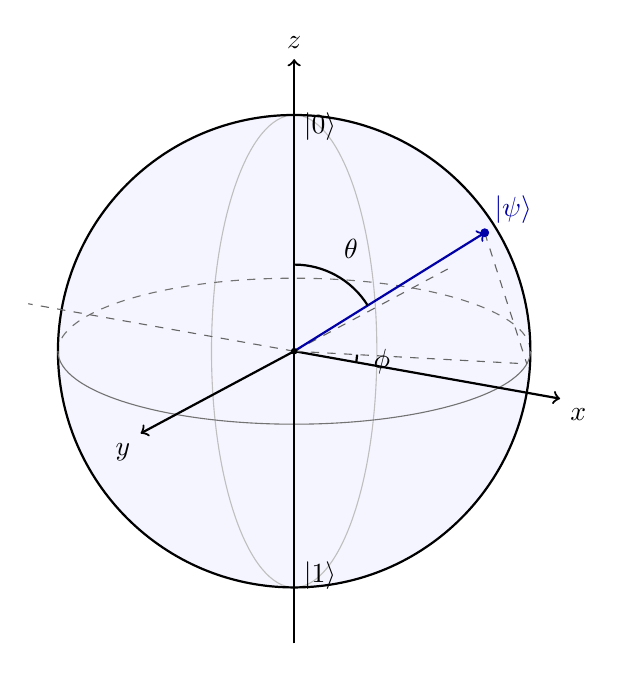
\begin{tikzpicture}

% ---------------- parameters ----------------
\pgfmathsetmacro{\SphR}{3}          % sphere radius
\pgfmathsetmacro{\SphRax}{3.9}      % axis arrow length (extends past the sphere)
\pgfmathsetmacro{\StTheta}{55}      % polar angle theta of |psi> (degrees from +z)
\pgfmathsetmacro{\StPhi}{-20}       % azimuthal angle phi of |psi> (degrees from +x)
\pgfmathsetmacro{\EqMinorR}{\SphR*sin(18)} % vertical semi-axis of the projected equator

\coordinate (O) at (0,0);

% axis tip / pole coordinates (on the sphere surface, radius \SphR)
\ProjectPoint{90}{0}{\SphR}{Xfront}
\ProjectPoint{90}{180}{\SphR}{Xback}
\ProjectPoint{90}{90}{\SphR}{Yfront}
\ProjectPoint{90}{270}{\SphR}{Yback}
\ProjectPoint{0}{0}{\SphR}{Ztop}
\ProjectPoint{180}{0}{\SphR}{Zbot}

% axis tip coordinates extended for the arrows/labels (radius \SphRax)
\ProjectPoint{90}{0}{\SphRax}{XfrontExt}
\ProjectPoint{90}{180}{\SphRax}{XbackExt}
\ProjectPoint{90}{90}{\SphRax}{YfrontExt}
\ProjectPoint{90}{270}{\SphRax}{YbackExt}
\ProjectPoint{0}{0}{\SphRax}{ZtopExt}
\ProjectPoint{180}{0}{\SphRax}{ZbotExt}

% the state vector |psi> and its shadow on the equatorial plane
\ProjectPoint{\StTheta}{\StPhi}{\SphR}{Psi}
\ProjectPoint{90}{\StPhi}{\SphR}{PsiShadow}

% ---------------- sphere body ----------------
\fill[blue!4] (O) circle (\SphR);

% a thin decorative meridian, purely to hint at the 3D volume
\draw[black!25,thin] (O) ellipse ({\SphR*0.35} and \SphR);

% equator: back half dashed, front half solid, main circle drawn on top
\draw[black!55,dashed] (\SphR,0) arc (0:180:{\SphR} and {\EqMinorR});
\draw[thick] (O) circle (\SphR);
\draw[black!55] (-\SphR,0) arc (180:360:{\SphR} and {\EqMinorR});

% ---------------- coordinate axes ----------------
% back (hidden) halves, dashed
\draw[dashed,black!60] (O) -- (XbackExt);
\draw[dashed,black!60] (O) -- (YbackExt);

% front (visible) halves, solid with arrowheads
\draw[thick,->] (O) -- (XfrontExt) node[below right] {$x$};
\draw[thick,->] (O) -- (YfrontExt) node[below left] {$y$};

% z axis: drawn as a single solid line (conventionally always visible)
\draw[thick,->] (ZbotExt) -- (ZtopExt) node[above] {$z$};

% pole labels
\node[right] at (Ztop) {$|0\rangle$};
\node[right] at (Zbot) {$|1\rangle$};

% ---------------- state vector |psi> ----------------
\draw[dashed,black!60] (O) -- (PsiShadow);
\draw[dashed,black!60] (Psi) -- (PsiShadow);

\draw[thick,->,blue!65!black] (O) -- (Psi);
\fill[blue!65!black] (Psi) circle (1.6pt);
\node[above right,blue!65!black] at (Psi) {$|\psi\rangle$};

% ---------------- angle arcs ----------------
\pic[draw, thick, angle radius=1.1cm, angle eccentricity=1.35, "$\theta$"]
  {angle = Psi--O--Ztop};
\pic[draw, thick, angle radius=0.8cm, angle eccentricity=1.4, "$\phi$"]
  {angle = Xfront--O--PsiShadow};

\fill (O) circle (1.2pt);

\end{tikzpicture}
\end{document}
